\documentclass[a4paper,11pt]{report}

%\usepackage{polski}
\usepackage[utf8]{inputenc}
\usepackage[OT4]{fontenc}
\usepackage[pdftex]{graphicx}

% Title Page
\title{nibblr}
\author{Michał Dettlaff \and Łukasz Draba \and Dariusz Kuziemski}
\date{\textsc{Uniwersytet Gdański, Maj 2011}}

\makeatletter
\newcommand{\linia}{\rule{\linewidth}{0.5mm}}
\renewcommand{\maketitle}{\begin{titlepage}
    \vspace*{5cm}
    \noindent\linia
    \begin{center} 
      \LARGE\textsc{\@title}
     \end{center}
     \linia
    \vspace{2cm}
    \begin{flushright}
    \begin{minipage}{5cm}
    \begin{tabular}[t]{l}%
    \@author
    \end{tabular}\par
    \end{minipage}
     \end{flushright}
    \vfill
    \begin{center}
    \@date
    \end{center}
  \end{titlepage}
}
\makeatother

\begin{document}
\maketitle

\section{Opis programu}

%D: jakiś wstęp, warto może jakąś ideę programu ładnie opisać - jak Michał
%opowiadał przed zajęciami
\subsection{Wstęp}
W erze wszechogarniającego internet bałaganu \textbf{nibblr} wychodzi naprzeciw
oczekiwaniom użytkowników i dzięki współpracy agentów wybiera dla niego to co go
interesuje. Nibblr (ze starourduńskiego ``dziobać'') %nie wiem ;)
po prostu wydziobuje to co jest istotne (warstwę danych?)

\begin{center}
 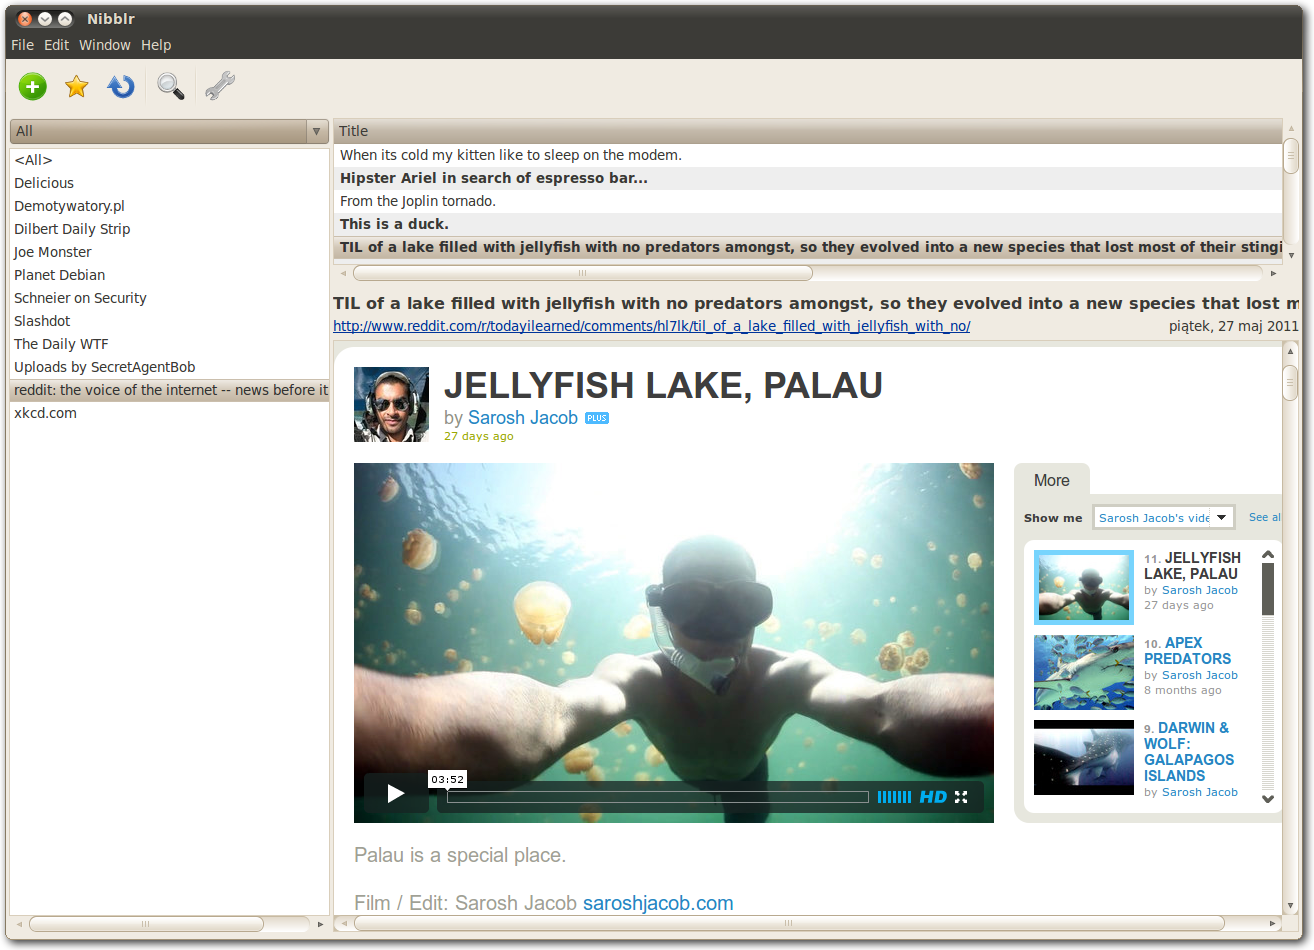
\includegraphics[scale=0.27]{./img/nibblr0.png}
\end{center}

%D: mam duże wątpliwości co do nazewnictwa ``subskrybowane kanały'' - brzmi jak
rss
%nie wiem czy nie przyczepi się jakoś do tego??
\newpage
\subsection{Opis interfejsu}

%D: można napisać że jest zrobiony w swt i że działa na linux/windows...

\begin{figure}[h]
 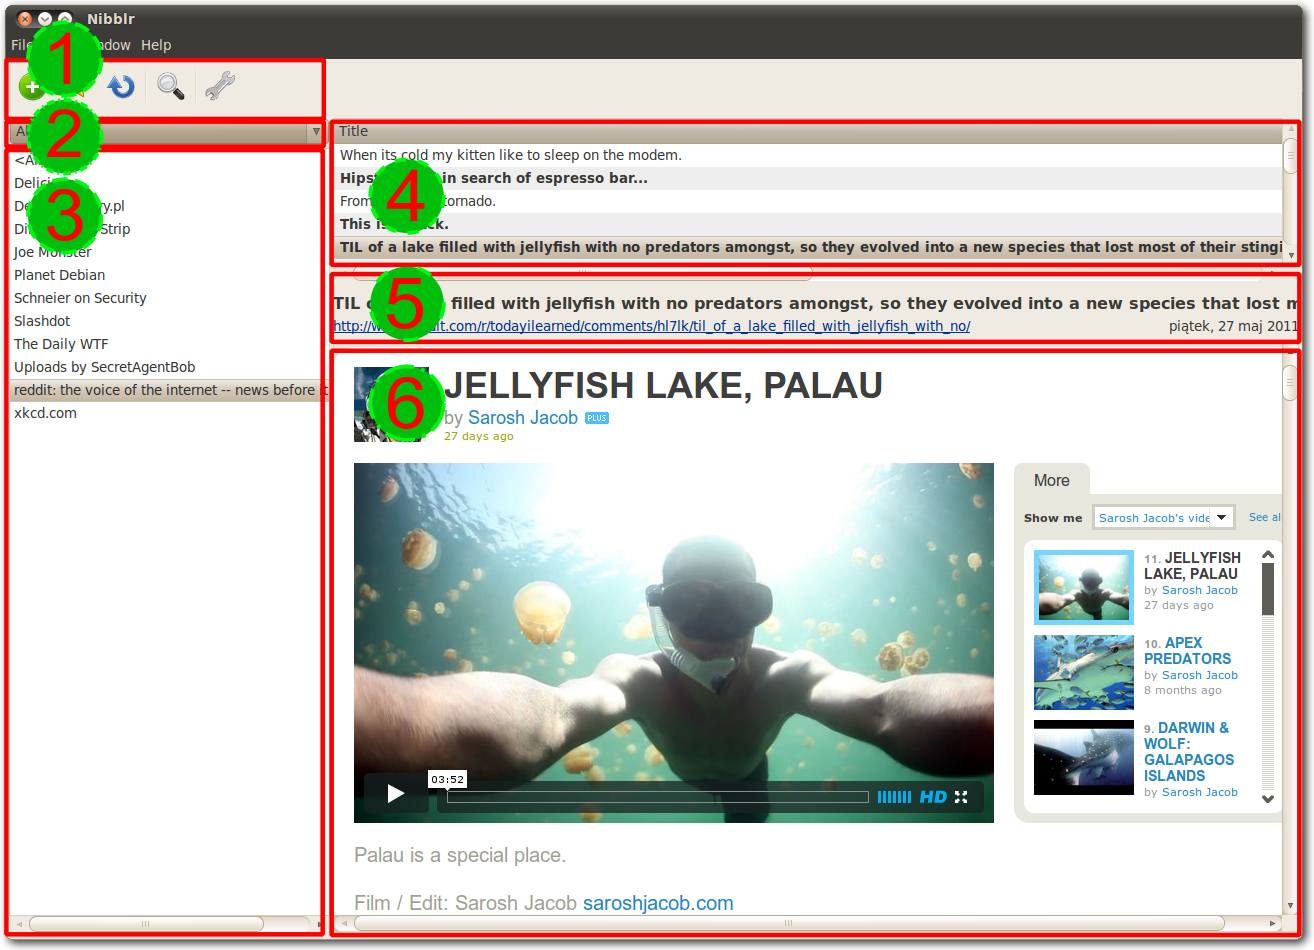
\includegraphics[scale=0.27]{./img/nibblr1.png}
 \caption{Interfejs główny programu nibblr można podzielić na 6 zasadniczych
części, kolejno: 
\newline \hspace* {1,5cm}1. Menu podręczne, 
\newline \hspace* {1,5cm}2. Filtrowanie według
przeczytane/nieprzeczytane/wszystkie, 
\newline \hspace* {1,5cm}3. Lista subskrypcji, 
\newline \hspace* {1,5cm}4. Dostępne feed'y
%feed'y?
\newline \hspace* {1,5cm}5. Informacje o aktualnym feed, 
\newline \hspace* {1,5cm}6. Treść feed'a
}
 \label{fig:interface6}
\end{figure}

\newpage
\subsubsection*{1. Menu podręczne}


\includegraphics[scale=0.8]{./img/menu.png}

\begin{itemize}

  \item[\textbf{Add}] - pozwala na dodanie kanału do listy aktualnie
  subskrybowanych, po kliknięciu na przycisk Add w menu pojawia się lista
  dostępnych subskrypcji
  \begin{center}
  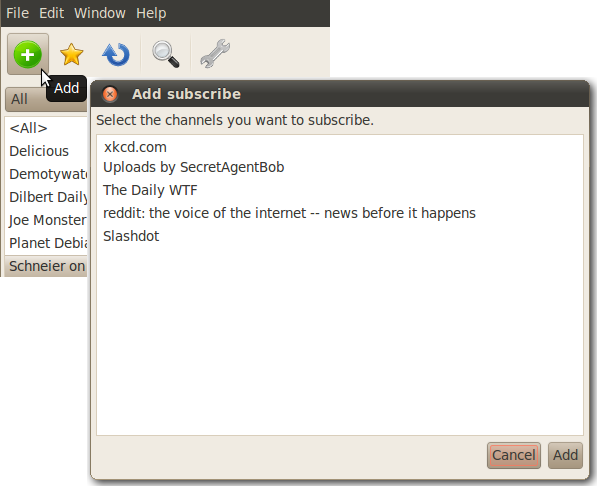
\includegraphics[scale=0.5]{./img/menu_add.png}
  \end{center}


  \item[\textbf{Recommend}] - pozwala na dodanie kanału z listy rekomendowanych
  %D: jak się to odbywa? To są te same co w Add?
  \begin{center}
  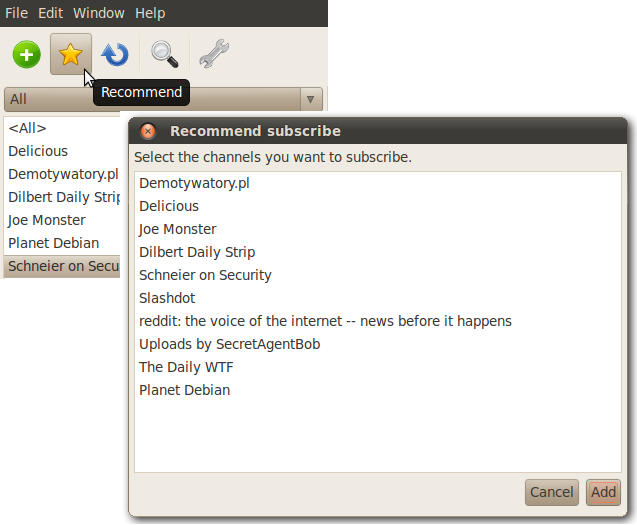
\includegraphics[scale=0.5]{./img/menu_recom.png}
  \end{center}


  \item[\textbf{Synchronize}] - Odświeża informacje z aktualnie subskrybowanych
  kanałów, po kliknięciu następuje sprawdzenie czy pojawiły się nowe feed'y,
  jeżeli tak - są automatycznie dodawane do listy
  \begin{center}
  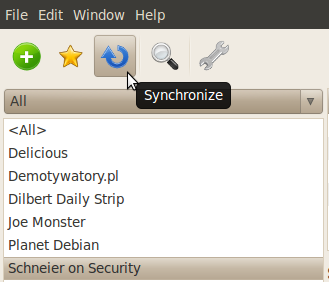
\includegraphics[scale=0.5]{./img/menu_sync.png}
  \end{center}

  \item[\textbf{Search}] - Przeszukanie feed'ów w poszukiwaniu słowa

  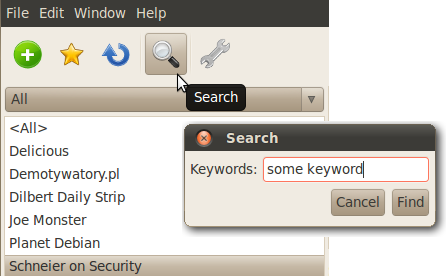
\includegraphics[scale=0.5]{./img/menu_search.png}


  %D: może pominąć?
  \item[\textbf{Preferences}] - Konfiguracja programu

  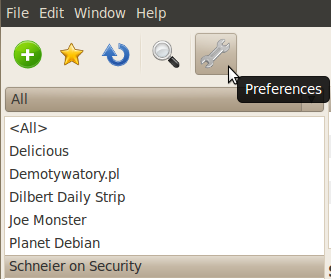
\includegraphics[scale=0.5]{./img/menu_pref.png}

\end{itemize}

\newpage
\subsubsection*{2. Filtrowanie według
przeczytane/nieprzeczytane/wszystkie}
Daje możliwość filtrowania feed'ów według tego czy zostały już przeczytanie,
wybór \textbf{All} wyłącza filtrowanie.

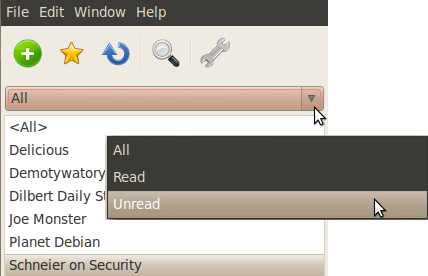
\includegraphics[scale=0.5]{./img/menu_readmenu1.png}

\subsubsection*{3. Lista subskrypcji}
%D: naprawde nie wiem co więcej by można napisać?
Tutaj widoczne są wszystkie zasubskrybowane kanały.

\subsubsection*{4. Dostępne feed'y}
Lista feed'ów z wybranej subskrypcji...

\subsection{5. Informacje o aktualnym feed}
Zawiera informacje takie jak data i odnośnik do feed.

\subsection{6. Treść feed'a}
%D: funkcjonalna przeglądarka (gdyby tylko dorobić pasek adresu, pełna
%konkurencja dla najnowszej wersji IE, trwają prace nad załączeniem adblocka ;-)
Tutaj pojawia się interesująca dla użytkownika treść.
%D: nie mam pomysłów na opisy, muszę się z tym wszystkim przespać, może na coś
%jeszcze wpadne...

\section{Diagram agentów}
%D: tu pewnie będzie jeden wielki diagram...


\section{Wizje przyszłościowe}

\end{document}          

